\documentclass[]{article}
\usepackage{lmodern}
\usepackage{amssymb,amsmath}
\usepackage{ifxetex,ifluatex}
\usepackage{fixltx2e} % provides \textsubscript
\ifnum 0\ifxetex 1\fi\ifluatex 1\fi=0 % if pdftex
  \usepackage[T1]{fontenc}
  \usepackage[utf8]{inputenc}
\else % if luatex or xelatex
  \ifxetex
    \usepackage{mathspec}
  \else
    \usepackage{fontspec}
  \fi
  \defaultfontfeatures{Ligatures=TeX,Scale=MatchLowercase}
\fi
% use upquote if available, for straight quotes in verbatim environments
\IfFileExists{upquote.sty}{\usepackage{upquote}}{}
% use microtype if available
\IfFileExists{microtype.sty}{%
\usepackage{microtype}
\UseMicrotypeSet[protrusion]{basicmath} % disable protrusion for tt fonts
}{}
\usepackage[margin=1in]{geometry}
\usepackage{hyperref}
\hypersetup{unicode=true,
            pdftitle={Assigment 4},
            pdfborder={0 0 0},
            breaklinks=true}
\urlstyle{same}  % don't use monospace font for urls
\usepackage{color}
\usepackage{fancyvrb}
\newcommand{\VerbBar}{|}
\newcommand{\VERB}{\Verb[commandchars=\\\{\}]}
\DefineVerbatimEnvironment{Highlighting}{Verbatim}{commandchars=\\\{\}}
% Add ',fontsize=\small' for more characters per line
\usepackage{framed}
\definecolor{shadecolor}{RGB}{248,248,248}
\newenvironment{Shaded}{\begin{snugshade}}{\end{snugshade}}
\newcommand{\AlertTok}[1]{\textcolor[rgb]{0.94,0.16,0.16}{#1}}
\newcommand{\AnnotationTok}[1]{\textcolor[rgb]{0.56,0.35,0.01}{\textbf{\textit{#1}}}}
\newcommand{\AttributeTok}[1]{\textcolor[rgb]{0.77,0.63,0.00}{#1}}
\newcommand{\BaseNTok}[1]{\textcolor[rgb]{0.00,0.00,0.81}{#1}}
\newcommand{\BuiltInTok}[1]{#1}
\newcommand{\CharTok}[1]{\textcolor[rgb]{0.31,0.60,0.02}{#1}}
\newcommand{\CommentTok}[1]{\textcolor[rgb]{0.56,0.35,0.01}{\textit{#1}}}
\newcommand{\CommentVarTok}[1]{\textcolor[rgb]{0.56,0.35,0.01}{\textbf{\textit{#1}}}}
\newcommand{\ConstantTok}[1]{\textcolor[rgb]{0.00,0.00,0.00}{#1}}
\newcommand{\ControlFlowTok}[1]{\textcolor[rgb]{0.13,0.29,0.53}{\textbf{#1}}}
\newcommand{\DataTypeTok}[1]{\textcolor[rgb]{0.13,0.29,0.53}{#1}}
\newcommand{\DecValTok}[1]{\textcolor[rgb]{0.00,0.00,0.81}{#1}}
\newcommand{\DocumentationTok}[1]{\textcolor[rgb]{0.56,0.35,0.01}{\textbf{\textit{#1}}}}
\newcommand{\ErrorTok}[1]{\textcolor[rgb]{0.64,0.00,0.00}{\textbf{#1}}}
\newcommand{\ExtensionTok}[1]{#1}
\newcommand{\FloatTok}[1]{\textcolor[rgb]{0.00,0.00,0.81}{#1}}
\newcommand{\FunctionTok}[1]{\textcolor[rgb]{0.00,0.00,0.00}{#1}}
\newcommand{\ImportTok}[1]{#1}
\newcommand{\InformationTok}[1]{\textcolor[rgb]{0.56,0.35,0.01}{\textbf{\textit{#1}}}}
\newcommand{\KeywordTok}[1]{\textcolor[rgb]{0.13,0.29,0.53}{\textbf{#1}}}
\newcommand{\NormalTok}[1]{#1}
\newcommand{\OperatorTok}[1]{\textcolor[rgb]{0.81,0.36,0.00}{\textbf{#1}}}
\newcommand{\OtherTok}[1]{\textcolor[rgb]{0.56,0.35,0.01}{#1}}
\newcommand{\PreprocessorTok}[1]{\textcolor[rgb]{0.56,0.35,0.01}{\textit{#1}}}
\newcommand{\RegionMarkerTok}[1]{#1}
\newcommand{\SpecialCharTok}[1]{\textcolor[rgb]{0.00,0.00,0.00}{#1}}
\newcommand{\SpecialStringTok}[1]{\textcolor[rgb]{0.31,0.60,0.02}{#1}}
\newcommand{\StringTok}[1]{\textcolor[rgb]{0.31,0.60,0.02}{#1}}
\newcommand{\VariableTok}[1]{\textcolor[rgb]{0.00,0.00,0.00}{#1}}
\newcommand{\VerbatimStringTok}[1]{\textcolor[rgb]{0.31,0.60,0.02}{#1}}
\newcommand{\WarningTok}[1]{\textcolor[rgb]{0.56,0.35,0.01}{\textbf{\textit{#1}}}}
\usepackage{graphicx,grffile}
\makeatletter
\def\maxwidth{\ifdim\Gin@nat@width>\linewidth\linewidth\else\Gin@nat@width\fi}
\def\maxheight{\ifdim\Gin@nat@height>\textheight\textheight\else\Gin@nat@height\fi}
\makeatother
% Scale images if necessary, so that they will not overflow the page
% margins by default, and it is still possible to overwrite the defaults
% using explicit options in \includegraphics[width, height, ...]{}
\setkeys{Gin}{width=\maxwidth,height=\maxheight,keepaspectratio}
\IfFileExists{parskip.sty}{%
\usepackage{parskip}
}{% else
\setlength{\parindent}{0pt}
\setlength{\parskip}{6pt plus 2pt minus 1pt}
}
\setlength{\emergencystretch}{3em}  % prevent overfull lines
\providecommand{\tightlist}{%
  \setlength{\itemsep}{0pt}\setlength{\parskip}{0pt}}
\setcounter{secnumdepth}{0}
% Redefines (sub)paragraphs to behave more like sections
\ifx\paragraph\undefined\else
\let\oldparagraph\paragraph
\renewcommand{\paragraph}[1]{\oldparagraph{#1}\mbox{}}
\fi
\ifx\subparagraph\undefined\else
\let\oldsubparagraph\subparagraph
\renewcommand{\subparagraph}[1]{\oldsubparagraph{#1}\mbox{}}
\fi

%%% Use protect on footnotes to avoid problems with footnotes in titles
\let\rmarkdownfootnote\footnote%
\def\footnote{\protect\rmarkdownfootnote}

%%% Change title format to be more compact
\usepackage{titling}

% Create subtitle command for use in maketitle
\providecommand{\subtitle}[1]{
  \posttitle{
    \begin{center}\large#1\end{center}
    }
}

\setlength{\droptitle}{-2em}

  \title{Assigment 4}
    \pretitle{\vspace{\droptitle}\centering\huge}
  \posttitle{\par}
    \author{}
    \preauthor{}\postauthor{}
    \date{}
    \predate{}\postdate{}
  

\begin{document}
\maketitle

\begin{enumerate}
\def\labelenumi{\arabic{enumi}.}
\tightlist
\item
  For the Boston data available in package MASS we wish to relate
  \texttt{dis} (weighted mean of distances to five Boston employment
  centres) to \texttt{nox} (nitrogen oxides concentration in parts per
  10 million).
\end{enumerate}

\begin{enumerate}
\def\labelenumi{(\alph{enumi})}
\tightlist
\item
  Fit a cubic polynomial to the data. Plot the data and the fit. Comment
  on the fit. Calculate the MSE.
\end{enumerate}

\begin{Shaded}
\begin{Highlighting}[]
\KeywordTok{library}\NormalTok{(tidyverse)}
\KeywordTok{library}\NormalTok{(MASS)}

\NormalTok{f1 <-}\StringTok{ }\KeywordTok{lm}\NormalTok{(dis }\OperatorTok{~}\StringTok{ }\KeywordTok{poly}\NormalTok{(nox,}\DecValTok{3}\NormalTok{), }\DataTypeTok{data =}\NormalTok{ Boston)}

\KeywordTok{ggplot}\NormalTok{(}\DataTypeTok{data=}\NormalTok{Boston, }\KeywordTok{aes}\NormalTok{(}\DataTypeTok{x=}\NormalTok{nox, }\DataTypeTok{y=}\NormalTok{dis)) }\OperatorTok{+}\StringTok{ }
\StringTok{  }\KeywordTok{geom_point}\NormalTok{() }\OperatorTok{+}\StringTok{ }
\StringTok{  }\KeywordTok{geom_line}\NormalTok{(}\KeywordTok{aes}\NormalTok{(}\DataTypeTok{y =} \KeywordTok{fitted}\NormalTok{(f1)), }\DataTypeTok{color =}\StringTok{"red"}\NormalTok{) }\OperatorTok{+}
\StringTok{  }\KeywordTok{theme_bw}\NormalTok{()}
\end{Highlighting}
\end{Shaded}

\begin{center}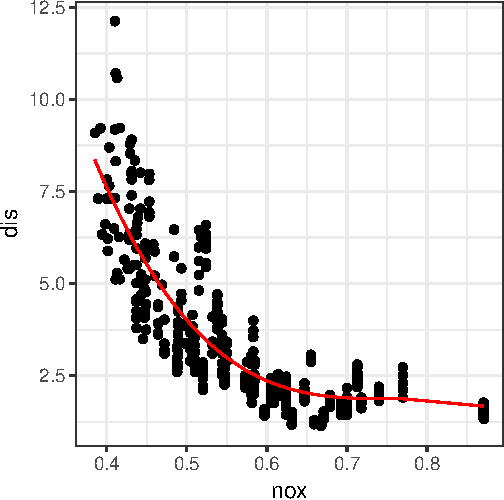
\includegraphics{sol_A4_files/figure-latex/unnamed-chunk-1-1} \end{center}

\begin{Shaded}
\begin{Highlighting}[]
\KeywordTok{mean}\NormalTok{(}\KeywordTok{residuals}\NormalTok{(f1)}\OperatorTok{^}\DecValTok{2}\NormalTok{)}
\end{Highlighting}
\end{Shaded}

\begin{verbatim}
## [1] 1.094805
\end{verbatim}

\begin{quote}
A reasonable fit. Residual plots show increasing variance. Very mild
curvature.
\end{quote}

\begin{enumerate}
\def\labelenumi{(\alph{enumi})}
\setcounter{enumi}{1}
\tightlist
\item
  Repeat (a), this time using a 10th degree polynomial. Compare the fits
  and the MSE. Use anova to compare the two fits and comment on your
  findings.
\end{enumerate}

\begin{Shaded}
\begin{Highlighting}[]
\NormalTok{f2 <-}\StringTok{ }\KeywordTok{lm}\NormalTok{(dis }\OperatorTok{~}\StringTok{ }\KeywordTok{poly}\NormalTok{(nox, }\DecValTok{10}\NormalTok{), }\DataTypeTok{data =}\NormalTok{ Boston)}

\KeywordTok{ggplot}\NormalTok{(}\DataTypeTok{data=}\NormalTok{Boston, }\KeywordTok{aes}\NormalTok{(}\DataTypeTok{x=}\NormalTok{nox, }\DataTypeTok{y=}\NormalTok{dis)) }\OperatorTok{+}\StringTok{ }
\StringTok{  }\KeywordTok{geom_point}\NormalTok{() }\OperatorTok{+}\StringTok{ }
\StringTok{  }\KeywordTok{geom_line}\NormalTok{(}\KeywordTok{aes}\NormalTok{(}\DataTypeTok{y =} \KeywordTok{fitted}\NormalTok{(f2)), }\DataTypeTok{color =} \StringTok{"blue"}\NormalTok{) }\OperatorTok{+}
\StringTok{  }\KeywordTok{theme_bw}\NormalTok{()}
\end{Highlighting}
\end{Shaded}

\begin{center}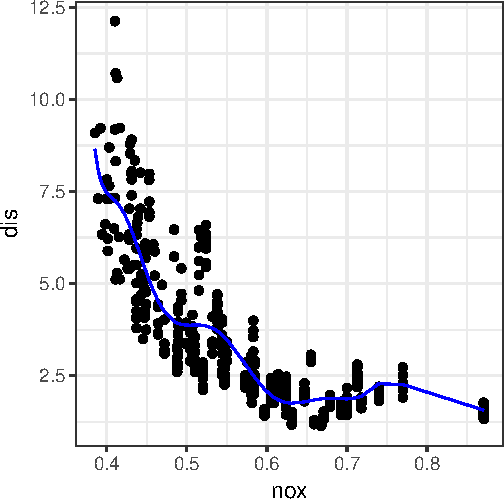
\includegraphics{sol_A4_files/figure-latex/unnamed-chunk-2-1} \end{center}

\begin{Shaded}
\begin{Highlighting}[]
\KeywordTok{mean}\NormalTok{(}\KeywordTok{residuals}\NormalTok{(f2)}\OperatorTok{^}\DecValTok{2}\NormalTok{)}
\end{Highlighting}
\end{Shaded}

\begin{verbatim}
## [1] 1.011485
\end{verbatim}

\begin{quote}
Some of the terms in f2 are significant (not all = 0). From the graph it
overfits the data, but picks up the increase in dis with increasing nox
past 0.65.
\end{quote}

\begin{enumerate}
\def\labelenumi{(\alph{enumi})}
\setcounter{enumi}{2}
\tightlist
\item
  Describe how you might use cross-validation to select the optimal
  degree (say between 1 and 10).
\end{enumerate}

Split the data into 5 groups of approximately equal size. for each
degree (j) between 1 and 10, - for each hold out sample, fit the model
on the rest and calculate the average test error on the hold out sample,
this gives mse1\ldots{} mse5. the cv error for degree j is the
(weighted) average of the mse1\ldots{}. mse5. Pick the degree with the
smallest cv error.

\begin{enumerate}
\def\labelenumi{(\alph{enumi})}
\setcounter{enumi}{3}
\tightlist
\item
  Carry out the cross-validation procedure. What is the optimal degree?
\end{enumerate}

\begin{Shaded}
\begin{Highlighting}[]
\KeywordTok{library}\NormalTok{(tidymodels)}
\KeywordTok{set.seed}\NormalTok{(}\DecValTok{2019}\NormalTok{)}

\KeywordTok{set.seed}\NormalTok{(}\DecValTok{2018}\NormalTok{)}
\NormalTok{cv_splits <-}\StringTok{ }\KeywordTok{vfold_cv}\NormalTok{(}
  \DataTypeTok{data =}\NormalTok{ Boston, }
  \DataTypeTok{v =} \DecValTok{5} 
\NormalTok{)}


\NormalTok{spec_lm <-}\StringTok{ }\KeywordTok{linear_reg}\NormalTok{() }\OperatorTok\StringTok{ }\KeywordTok{set_engine}\NormalTok{(}\StringTok{"lm"}\NormalTok{)}

\NormalTok{geo_form <-}\StringTok{ }\NormalTok{dis }\OperatorTok{~}\StringTok{ }\KeywordTok{poly}\NormalTok{(nox, }\DecValTok{3}\NormalTok{)}

\NormalTok{fit_model <-}\StringTok{ }\ControlFlowTok{function}\NormalTok{(split, spec) \{}
  \KeywordTok{fit}\NormalTok{(}
    \DataTypeTok{object =}\NormalTok{ spec, }
    \DataTypeTok{formula =}\NormalTok{ geo_form,}
    \DataTypeTok{data =} \KeywordTok{analysis}\NormalTok{(split) }
\NormalTok{  )}
\NormalTok{\}  }

\NormalTok{compute_pred <-}\StringTok{ }\ControlFlowTok{function}\NormalTok{(split, model) \{}
  \CommentTok{# Extract the assessment set}
\NormalTok{  assess <-}\StringTok{ }\KeywordTok{assessment}\NormalTok{(split) }
  \CommentTok{# Compute predictions (a df is returned)}
\NormalTok{  pred <-}\StringTok{ }\KeywordTok{predict}\NormalTok{(model, }\DataTypeTok{new_data =}\NormalTok{ assess)}
  \KeywordTok{bind_cols}\NormalTok{(assess, pred)}
\NormalTok{\}}

\NormalTok{compute_perf <-}\StringTok{ }\ControlFlowTok{function}\NormalTok{(pred_df) \{}
\NormalTok{  numeric_metrics <-}\StringTok{ }\KeywordTok{metric_set}\NormalTok{(rmse, rsq)}
  
  \KeywordTok{numeric_metrics}\NormalTok{(}
\NormalTok{    pred_df, }
    \DataTypeTok{truth =}\NormalTok{ dis, }
    \DataTypeTok{estimate =}\NormalTok{ .pred}
\NormalTok{  )}
\NormalTok{\}}


\NormalTok{mse_cv <-}\StringTok{ }\ControlFlowTok{function}\NormalTok{(degree)\{}
  
\NormalTok{  geo_form <-}\StringTok{ }\NormalTok{dis }\OperatorTok{~}\StringTok{ }\KeywordTok{poly}\NormalTok{(nox, degree)}
  
\NormalTok{  fit_model <-}\StringTok{ }\ControlFlowTok{function}\NormalTok{(split, spec) \{}
    \KeywordTok{fit}\NormalTok{(}
      \DataTypeTok{object =}\NormalTok{ spec, }
      \DataTypeTok{formula =}\NormalTok{ geo_form,}
      \DataTypeTok{data =} \KeywordTok{analysis}\NormalTok{(split) }
\NormalTok{    )}
\NormalTok{  \}  }
  
  
\NormalTok{  cv_splits <-}\StringTok{ }\NormalTok{cv_splits }\OperatorTok\StringTok{ }
\StringTok{    }\KeywordTok{mutate}\NormalTok{(}\DataTypeTok{models_lm =} \KeywordTok{map}\NormalTok{(splits, fit_model, spec_lm),}
           \DataTypeTok{pred_lm =} \KeywordTok{map2}\NormalTok{(splits, models_lm, compute_pred),}
           \DataTypeTok{perf =} \KeywordTok{map}\NormalTok{(pred_lm, compute_perf))}
  
\NormalTok{  cv_splits }\OperatorTok\StringTok{ }
\StringTok{    }\KeywordTok{unnest}\NormalTok{(perf) }\OperatorTok\StringTok{ }
\StringTok{    }\KeywordTok{filter}\NormalTok{(.metric }\OperatorTok{==}\StringTok{ 'rmse'}\NormalTok{) }\OperatorTok\StringTok{ }
\StringTok{    }\KeywordTok{summarise}\NormalTok{(}\DataTypeTok{m =} \KeywordTok{mean}\NormalTok{(.estimate)) }\OperatorTok\StringTok{ }
\StringTok{    }\KeywordTok{pull}\NormalTok{(m)}
  
\NormalTok{\}}

\NormalTok{mses <-}\StringTok{ }\KeywordTok{data.frame}\NormalTok{(}\DataTypeTok{rmse =} \DecValTok{1}\OperatorTok{:}\DecValTok{10} \OperatorTok\StringTok{ }\KeywordTok{map_dbl}\NormalTok{(mse_cv),}
                   \DataTypeTok{deg =} \DecValTok{1}\OperatorTok{:}\DecValTok{10}\NormalTok{)}

\NormalTok{mses }\OperatorTok\StringTok{ }
\StringTok{  }\KeywordTok{ggplot}\NormalTok{(}\KeywordTok{aes}\NormalTok{(}\DataTypeTok{y =}\NormalTok{ rmse, }\KeywordTok{factor}\NormalTok{(deg), }\DataTypeTok{group =} \DecValTok{1}\NormalTok{)) }\OperatorTok{+}
\StringTok{  }\KeywordTok{geom_line}\NormalTok{() }\OperatorTok{+}
\StringTok{  }\KeywordTok{geom_point}\NormalTok{(}\DataTypeTok{colour =} \StringTok{"tomato"}\NormalTok{, }\DataTypeTok{size =} \DecValTok{2}\NormalTok{) }\OperatorTok{+}
\StringTok{  }\KeywordTok{theme_bw}\NormalTok{()}
\end{Highlighting}
\end{Shaded}

\begin{center}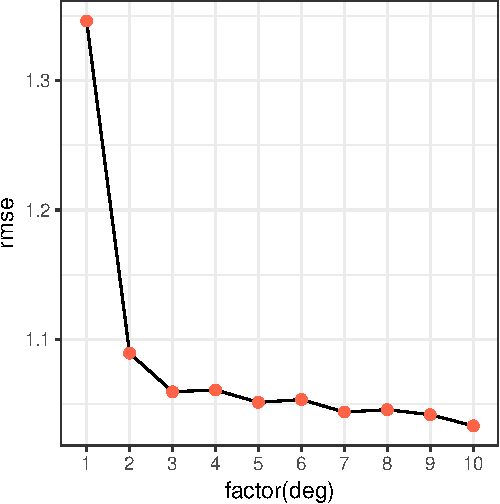
\includegraphics{sol_A4_files/figure-latex/unnamed-chunk-3-1} \end{center}

\begin{Shaded}
\begin{Highlighting}[]
\KeywordTok{which.min}\NormalTok{(mses}\OperatorTok{$}\NormalTok{rmse)}
\end{Highlighting}
\end{Shaded}

\begin{verbatim}
## [1] 10
\end{verbatim}

\begin{enumerate}
\def\labelenumi{(\alph{enumi})}
\setcounter{enumi}{4}
\tightlist
\item
  Use bs() to fit a regression spline with 4 degrees of freedom. What
  are the knots used? Plot the data and the fit. Comment on the fit.
  Calculate the MSE.
\end{enumerate}

\begin{Shaded}
\begin{Highlighting}[]
\KeywordTok{library}\NormalTok{(splines)}
\NormalTok{f3 <-}\StringTok{ }\KeywordTok{lm}\NormalTok{(dis }\OperatorTok{~}\StringTok{ }\KeywordTok{bs}\NormalTok{(nox, }\DataTypeTok{df =} \DecValTok{4}\NormalTok{), }\DataTypeTok{data =}\NormalTok{ Boston)}
\KeywordTok{attr}\NormalTok{(}\KeywordTok{bs}\NormalTok{(Boston}\OperatorTok{$}\NormalTok{nox, }\DataTypeTok{df =} \DecValTok{4}\NormalTok{), }\StringTok{"knots"}\NormalTok{)}
\end{Highlighting}
\end{Shaded}

\begin{verbatim}
##   50% 
## 0.538
\end{verbatim}

\begin{Shaded}
\begin{Highlighting}[]
\NormalTok{Boston }\OperatorTok\StringTok{ }
\KeywordTok{ggplot}\NormalTok{(}\KeywordTok{aes}\NormalTok{(}\DataTypeTok{x =}\NormalTok{ nox, }\DataTypeTok{y =}\NormalTok{ dis)) }\OperatorTok{+}
\StringTok{  }\KeywordTok{geom_point}\NormalTok{() }\OperatorTok{+}\StringTok{ }
\StringTok{  }\KeywordTok{geom_line}\NormalTok{(}\KeywordTok{aes}\NormalTok{(}\DataTypeTok{y =} \KeywordTok{fitted}\NormalTok{(f3)), }\DataTypeTok{color =} \StringTok{"red"}\NormalTok{) }\OperatorTok{+}
\StringTok{  }\KeywordTok{theme_bw}\NormalTok{()}
\end{Highlighting}
\end{Shaded}

\begin{center}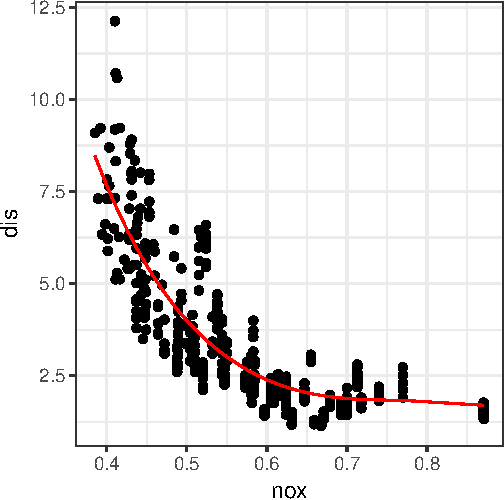
\includegraphics{sol_A4_files/figure-latex/unnamed-chunk-4-1} \end{center}

\begin{Shaded}
\begin{Highlighting}[]
\KeywordTok{sqrt}\NormalTok{(}\KeywordTok{mean}\NormalTok{(}\KeywordTok{residuals}\NormalTok{(f3)}\OperatorTok{^}\DecValTok{2}\NormalTok{))}
\end{Highlighting}
\end{Shaded}

\begin{verbatim}
## [1] 1.046016
\end{verbatim}

\begin{enumerate}
\def\labelenumi{(\alph{enumi})}
\setcounter{enumi}{5}
\tightlist
\item
  Fit a curve using a smoothing spline with the automatically chosen
  amount of smoothing. Display the fit. Does the automatic \(\lambda\)
  give a good result?
\end{enumerate}

\begin{Shaded}
\begin{Highlighting}[]
\NormalTok{f4 <-}\StringTok{ }\KeywordTok{smooth.spline}\NormalTok{(Boston}\OperatorTok{$}\NormalTok{nox, Boston}\OperatorTok{$}\NormalTok{dis, }\DataTypeTok{cv =} \OtherTok{TRUE}\NormalTok{)}
\NormalTok{f4}
\end{Highlighting}
\end{Shaded}

\begin{verbatim}
## Call:
## smooth.spline(x = Boston$nox, y = Boston$dis, cv = TRUE)
## 
## Smoothing Parameter  spar= 1.050661  lambda= 0.07031691 (16 iterations)
## Equivalent Degrees of Freedom (Df): 4.128915
## Penalized Criterion (RSS): 407.277
## PRESS(l.o.o. CV): 1.119355
\end{verbatim}

\begin{Shaded}
\begin{Highlighting}[]
\NormalTok{Boston }\OperatorTok\StringTok{ }
\KeywordTok{ggplot}\NormalTok{(}\KeywordTok{aes}\NormalTok{(}\DataTypeTok{x =}\NormalTok{ nox, }\DataTypeTok{y =}\NormalTok{ dis)) }\OperatorTok{+}\StringTok{ }
\StringTok{  }\KeywordTok{geom_point}\NormalTok{() }\OperatorTok{+}\StringTok{ }
\StringTok{  }\KeywordTok{geom_line}\NormalTok{(}\KeywordTok{aes}\NormalTok{(}\DataTypeTok{y =} \KeywordTok{fitted}\NormalTok{(f4)), }\DataTypeTok{color =} \StringTok{"red"}\NormalTok{) }\OperatorTok{+}
\StringTok{  }\KeywordTok{theme_bw}\NormalTok{()}
\end{Highlighting}
\end{Shaded}

\begin{center}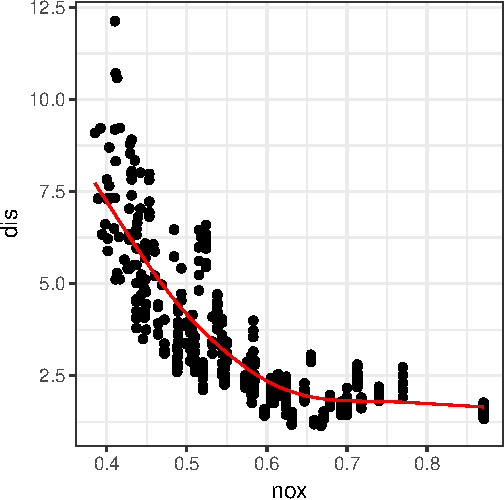
\includegraphics{sol_A4_files/figure-latex/unnamed-chunk-5-1} \end{center}

\begin{Shaded}
\begin{Highlighting}[]
\KeywordTok{sqrt}\NormalTok{(}\KeywordTok{mean}\NormalTok{(}\KeywordTok{residuals}\NormalTok{(f4)}\OperatorTok{^}\DecValTok{2}\NormalTok{))}
\end{Highlighting}
\end{Shaded}

\begin{verbatim}
## [1] 1.050964
\end{verbatim}

\begin{enumerate}
\def\labelenumi{(\alph{enumi})}
\setcounter{enumi}{6}
\tightlist
\item
  Now use smoothing spline with a larger value of spar. Overlay both
  smoothing spline fits on the plot. Which looks better?
\end{enumerate}

\begin{Shaded}
\begin{Highlighting}[]
\NormalTok{f5 <-}\StringTok{ }\KeywordTok{smooth.spline}\NormalTok{(Boston}\OperatorTok{$}\NormalTok{nox,Boston}\OperatorTok{$}\NormalTok{dis, }\DataTypeTok{spar =} \DecValTok{2}\NormalTok{)}
\NormalTok{f5}
\end{Highlighting}
\end{Shaded}

\begin{verbatim}
## Call:
## smooth.spline(x = Boston$nox, y = Boston$dis, spar = 2)
## 
## Smoothing Parameter  spar= 2  lambda= 508171.7
## Equivalent Degrees of Freedom (Df): 1.999947
## Penalized Criterion (RSS): 762.6087
## GCV: 1.82113
\end{verbatim}

\begin{Shaded}
\begin{Highlighting}[]
\NormalTok{Boston }\OperatorTok\StringTok{ }
\StringTok{  }\KeywordTok{ggplot}\NormalTok{(}\KeywordTok{aes}\NormalTok{(}\DataTypeTok{x =}\NormalTok{ nox, }\DataTypeTok{y =}\NormalTok{ dis))}\OperatorTok{+}\StringTok{ }\KeywordTok{geom_point}\NormalTok{() }\OperatorTok{+}\StringTok{ }
\StringTok{  }\KeywordTok{geom_line}\NormalTok{(}\KeywordTok{aes}\NormalTok{(}\DataTypeTok{y =} \KeywordTok{fitted}\NormalTok{(f4)), }\DataTypeTok{color =} \StringTok{"red"}\NormalTok{)}\OperatorTok{+}\StringTok{ }
\StringTok{  }\KeywordTok{geom_line}\NormalTok{(}\KeywordTok{aes}\NormalTok{(}\DataTypeTok{y =} \KeywordTok{fitted}\NormalTok{(f5)), }\DataTypeTok{color =} \StringTok{"blue"}\NormalTok{) }\OperatorTok{+}
\StringTok{  }\KeywordTok{theme_bw}\NormalTok{()}
\end{Highlighting}
\end{Shaded}

\begin{center}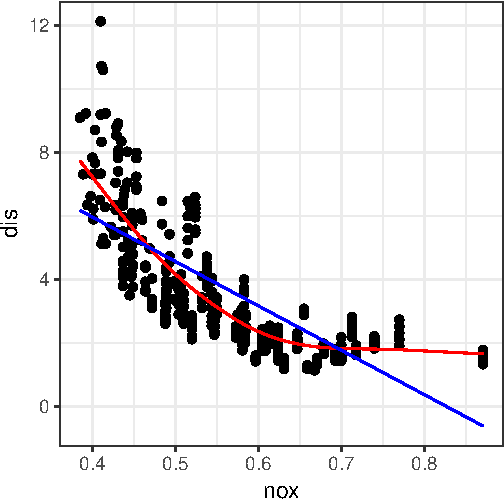
\includegraphics{sol_A4_files/figure-latex/unnamed-chunk-6-1} \end{center}

\begin{enumerate}
\def\labelenumi{\arabic{enumi}.}
\setcounter{enumi}{1}
\tightlist
\item
  Using the Boston data, with \texttt{dis} as the response and
  predictors \texttt{medv}, \texttt{age} and \texttt{nox}.
\end{enumerate}

\begin{enumerate}
\def\labelenumi{(\alph{enumi})}
\tightlist
\item
  Split the data into training 60\% and test 40\%. Using the training
  data, fit a generalised additive model (GAM). Use ns with 4 degrees of
  freedom for each predictor.
\end{enumerate}

\begin{Shaded}
\begin{Highlighting}[]
\KeywordTok{library}\NormalTok{(splines)}

\NormalTok{Boston <-}\StringTok{  }\NormalTok{Boston }\OperatorTok\StringTok{ }
\StringTok{  }\KeywordTok{mutate}\NormalTok{(}\DataTypeTok{part =} \KeywordTok{ifelse}\NormalTok{(}\KeywordTok{runif}\NormalTok{(}\KeywordTok{nrow}\NormalTok{(.)) }\OperatorTok{>}\StringTok{ }\FloatTok{0.6}\NormalTok{, }\StringTok{"test"}\NormalTok{, }\StringTok{"train"}\NormalTok{))}

\NormalTok{Boston }\OperatorTok\StringTok{ }
\StringTok{  }\NormalTok{janitor}\OperatorTok{::}\KeywordTok{tabyl}\NormalTok{(part)}
\end{Highlighting}
\end{Shaded}

\begin{verbatim}
##   part   n   percent
##   test 189 0.3735178
##  train 317 0.6264822
\end{verbatim}

\begin{Shaded}
\begin{Highlighting}[]
\NormalTok{train <-}\StringTok{ }\NormalTok{Boston }\OperatorTok\StringTok{ }\KeywordTok{filter}\NormalTok{(part }\OperatorTok{==}\StringTok{ "train"}\NormalTok{) }\OperatorTok\StringTok{ }\NormalTok{dplyr}\OperatorTok{::}\KeywordTok{select}\NormalTok{(}\OperatorTok{-}\NormalTok{part)}
\NormalTok{test <-}\StringTok{ }\NormalTok{Boston }\OperatorTok\StringTok{ }\KeywordTok{filter}\NormalTok{(part }\OperatorTok{==}\StringTok{ "test"}\NormalTok{) }\OperatorTok\StringTok{ }\NormalTok{dplyr}\OperatorTok{::}\KeywordTok{select}\NormalTok{(}\OperatorTok{-}\NormalTok{part)}

\NormalTok{gfit1 <-}\StringTok{  }\KeywordTok{lm}\NormalTok{(dis }\OperatorTok{~}\StringTok{ }\KeywordTok{ns}\NormalTok{(medv, }\DecValTok{4}\NormalTok{)}\OperatorTok{+}\StringTok{ }\KeywordTok{ns}\NormalTok{(age, }\DecValTok{4}\NormalTok{) }\OperatorTok{+}\StringTok{ }\KeywordTok{ns}\NormalTok{(nox, }\DecValTok{4}\NormalTok{), }\DataTypeTok{data =}\NormalTok{ train)}

\KeywordTok{pairs}\NormalTok{(Boston[, }\KeywordTok{c}\NormalTok{(}\DecValTok{8}\NormalTok{, }\DecValTok{7}\NormalTok{, }\DecValTok{5}\NormalTok{, }\DecValTok{14}\NormalTok{)])}
\end{Highlighting}
\end{Shaded}

\begin{center}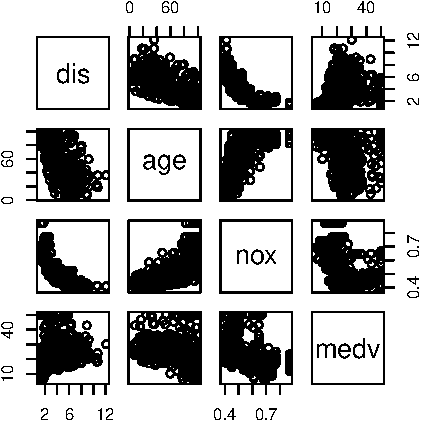
\includegraphics{sol_A4_files/figure-latex/unnamed-chunk-7-1} \end{center}

\begin{enumerate}
\def\labelenumi{(\alph{enumi})}
\setcounter{enumi}{1}
\tightlist
\item
  Use plot.gam to display the results. Does it appear if a linear term
  is appropriate for any of the predictors?
\end{enumerate}

\begin{Shaded}
\begin{Highlighting}[]
\KeywordTok{par}\NormalTok{(}\DataTypeTok{mfrow =} \KeywordTok{c}\NormalTok{(}\DecValTok{1}\NormalTok{, }\DecValTok{3}\NormalTok{))}
\NormalTok{gam}\OperatorTok{::}\KeywordTok{plot.Gam}\NormalTok{(gfit1)}
\end{Highlighting}
\end{Shaded}

\begin{center}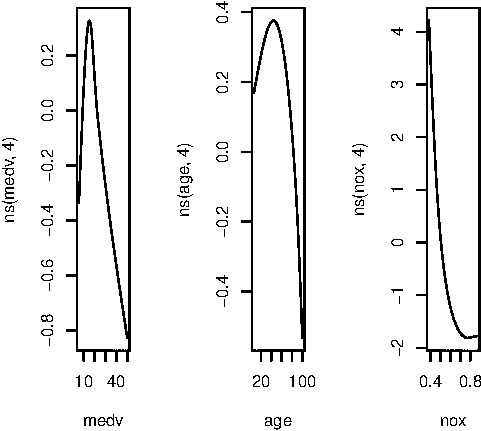
\includegraphics{sol_A4_files/figure-latex/unnamed-chunk-8-1} \end{center}

\begin{quote}
The linear model does not seem appropriate.
\end{quote}

\begin{enumerate}
\def\labelenumi{(\alph{enumi})}
\setcounter{enumi}{2}
\tightlist
\item
  Simplify the model fit in part (a). Refit the model. Use anova to
  compare the two fits and comment on your results.
\end{enumerate}

\begin{Shaded}
\begin{Highlighting}[]
\KeywordTok{attr}\NormalTok{(}\KeywordTok{ns}\NormalTok{(train}\OperatorTok{$}\NormalTok{age, }\DecValTok{4}\NormalTok{), }\StringTok{"knots"}\NormalTok{)}
\end{Highlighting}
\end{Shaded}

\begin{verbatim}
##  25%  50%  75% 
## 45.4 79.7 94.5
\end{verbatim}

\begin{Shaded}
\begin{Highlighting}[]
\KeywordTok{attr}\NormalTok{(}\KeywordTok{ns}\NormalTok{(train}\OperatorTok{$}\NormalTok{age, }\DecValTok{2}\NormalTok{), }\StringTok{"knots"}\NormalTok{)}
\end{Highlighting}
\end{Shaded}

\begin{verbatim}
##  50% 
## 79.7
\end{verbatim}

\begin{Shaded}
\begin{Highlighting}[]
\NormalTok{gfit2 <-}\StringTok{  }\KeywordTok{lm}\NormalTok{(dis }\OperatorTok{~}\StringTok{ }\KeywordTok{ns}\NormalTok{(medv, }\DecValTok{2}\NormalTok{) }\OperatorTok{+}\StringTok{ }\KeywordTok{ns}\NormalTok{(age, }\DecValTok{2}\NormalTok{) }\OperatorTok{+}\StringTok{ }\KeywordTok{ns}\NormalTok{(nox, }\DecValTok{2}\NormalTok{), }\DataTypeTok{data =}\NormalTok{ train)}

\KeywordTok{par}\NormalTok{(}\DataTypeTok{mfrow=}\KeywordTok{c}\NormalTok{(}\DecValTok{1}\NormalTok{,}\DecValTok{3}\NormalTok{))}
\NormalTok{gam}\OperatorTok{::}\KeywordTok{plot.Gam}\NormalTok{(gfit2)}
\end{Highlighting}
\end{Shaded}

\begin{center}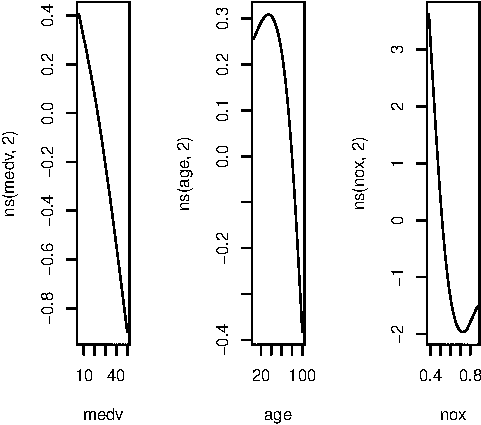
\includegraphics{sol_A4_files/figure-latex/unnamed-chunk-9-1} \end{center}

\begin{Shaded}
\begin{Highlighting}[]
\KeywordTok{anova}\NormalTok{(gfit1, gfit2)}
\end{Highlighting}
\end{Shaded}

\begin{verbatim}
## Analysis of Variance Table
## 
## Model 1: dis ~ ns(medv, 4) + ns(age, 4) + ns(nox, 4)
## Model 2: dis ~ ns(medv, 2) + ns(age, 2) + ns(nox, 2)
##   Res.Df    RSS Df Sum of Sq      F  Pr(>F)  
## 1    304 260.44                              
## 2    310 274.64 -6   -14.203 2.7631 0.01248 *
## ---
## Signif. codes:  0 '***' 0.001 '**' 0.01 '*' 0.05 '.' 0.1 ' ' 1
\end{verbatim}

\begin{quote}
the model with fewer df is not appropriate.
\end{quote}

\begin{enumerate}
\def\labelenumi{\arabic{enumi}.}
\setcounter{enumi}{3}
\item
\end{enumerate}

\begin{enumerate}
\def\labelenumi{(\alph{enumi})}
\tightlist
\item
  For the training data in question 2, fit a tree model. Use dis as
  response, and predictors \texttt{medv}, \texttt{age} and \texttt{nox}.
  Draw the tree. Calculate the training and test MSE.
\end{enumerate}

\begin{Shaded}
\begin{Highlighting}[]
\KeywordTok{library}\NormalTok{(tree)}
\NormalTok{tree <-}\StringTok{ }\KeywordTok{tree}\NormalTok{(dis }\OperatorTok{~}\StringTok{ }\NormalTok{medv }\OperatorTok{+}\StringTok{ }\NormalTok{age }\OperatorTok{+}\StringTok{ }\NormalTok{nox, }\DataTypeTok{data =}\NormalTok{ train)}
\KeywordTok{summary}\NormalTok{(tree)}
\end{Highlighting}
\end{Shaded}

\begin{verbatim}
## 
## Regression tree:
## tree(formula = dis ~ medv + age + nox, data = train)
## Number of terminal nodes:  9 
## Residual mean deviance:  0.5356 = 165 / 308 
## Distribution of residuals:
##     Min.  1st Qu.   Median     Mean  3rd Qu.     Max. 
## -2.10400 -0.42980 -0.06625  0.00000  0.38060  3.29900
\end{verbatim}

\begin{quote}
The fitted tree has 5 leaf nodes.
\end{quote}

\begin{Shaded}
\begin{Highlighting}[]
\KeywordTok{plot}\NormalTok{(tree)}
\KeywordTok{text}\NormalTok{(tree, }\DataTypeTok{cex =} \FloatTok{0.5}\NormalTok{, }\DataTypeTok{pretty =} \DecValTok{0}\NormalTok{)}
\end{Highlighting}
\end{Shaded}

\begin{center}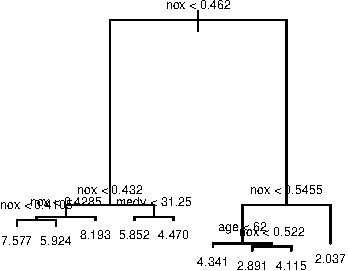
\includegraphics{sol_A4_files/figure-latex/unnamed-chunk-11-1} \end{center}

\begin{Shaded}
\begin{Highlighting}[]
\KeywordTok{sqrt}\NormalTok{(}\KeywordTok{mean}\NormalTok{(}\KeywordTok{residuals}\NormalTok{(tree)}\OperatorTok{^}\DecValTok{2}\NormalTok{))}
\end{Highlighting}
\end{Shaded}

\begin{verbatim}
## [1] 0.7213952
\end{verbatim}

\begin{Shaded}
\begin{Highlighting}[]
\NormalTok{pred <-}\StringTok{ }\KeywordTok{predict}\NormalTok{(tree, test)}
\KeywordTok{sqrt}\NormalTok{(}\KeywordTok{mean}\NormalTok{((test}\OperatorTok{$}\NormalTok{dis }\OperatorTok{-}\StringTok{ }\NormalTok{pred)}\OperatorTok{^}\DecValTok{2}\NormalTok{))}
\end{Highlighting}
\end{Shaded}

\begin{verbatim}
## [1] 1.199322
\end{verbatim}

\begin{enumerate}
\def\labelenumi{(\alph{enumi})}
\setcounter{enumi}{1}
\tightlist
\item
  Use \texttt{cv.tree} to select a pruned tree. If pruning is required,
  fit and draw the pruned tree. Calculate the training and test MSE.
  Compare the results to those in (a).
\end{enumerate}

\begin{Shaded}
\begin{Highlighting}[]
\NormalTok{cvtree <-}\StringTok{ }\KeywordTok{cv.tree}\NormalTok{(tree)}
\NormalTok{cvtree}
\end{Highlighting}
\end{Shaded}

\begin{verbatim}
## $size
## [1] 9 8 6 4 3 2 1
## 
## $dev
## [1]  266.0019  267.2256  277.7006  285.8440  325.2640  508.1814 1341.4652
## 
## $k
## [1]      -Inf  14.31800  16.52661  20.31122  54.70596 175.73910 854.63983
## 
## $method
## [1] "deviance"
## 
## attr(,"class")
## [1] "prune"         "tree.sequence"
\end{verbatim}

\begin{Shaded}
\begin{Highlighting}[]
\KeywordTok{ggplot}\NormalTok{() }\OperatorTok{+}
\StringTok{  }\KeywordTok{geom_point}\NormalTok{(}\KeywordTok{aes}\NormalTok{(}\DataTypeTok{x =} \KeywordTok{length}\NormalTok{(}\KeywordTok{c}\NormalTok{(cvtree}\OperatorTok{$}\NormalTok{dev))}\OperatorTok{:}\DecValTok{1}\NormalTok{, }\DataTypeTok{y =} \KeywordTok{c}\NormalTok{(cvtree}\OperatorTok{$}\NormalTok{dev))) }\OperatorTok{+}
\StringTok{  }\KeywordTok{geom_line}\NormalTok{(}\KeywordTok{aes}\NormalTok{(}\DataTypeTok{x =} \KeywordTok{length}\NormalTok{(}\KeywordTok{c}\NormalTok{(cvtree}\OperatorTok{$}\NormalTok{dev))}\OperatorTok{:}\DecValTok{1}\NormalTok{, }\DataTypeTok{y =} \KeywordTok{c}\NormalTok{(cvtree}\OperatorTok{$}\NormalTok{dev))) }\OperatorTok{+}
\StringTok{  }\KeywordTok{theme_bw}\NormalTok{()}
\end{Highlighting}
\end{Shaded}

\begin{center}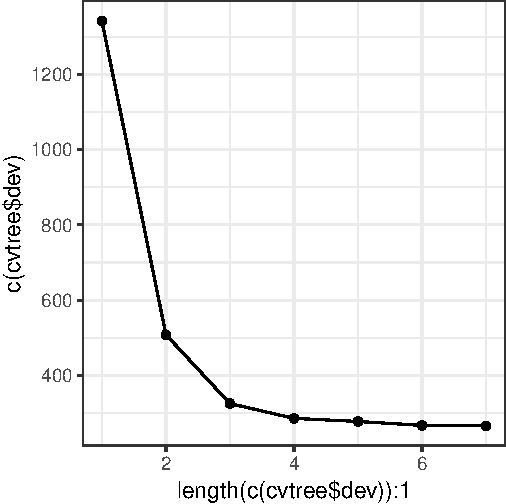
\includegraphics{sol_A4_files/figure-latex/unnamed-chunk-12-1} \end{center}

\begin{enumerate}
\def\labelenumi{(\alph{enumi})}
\setcounter{enumi}{2}
\tightlist
\item
  Which fit is better, the (optionally pruned) tree or the GAM? Compare
  their performance on the test data.
\end{enumerate}

\begin{Shaded}
\begin{Highlighting}[]
\NormalTok{pred <-}\StringTok{ }\KeywordTok{predict}\NormalTok{(tree, test)}
\KeywordTok{sqrt}\NormalTok{(}\KeywordTok{mean}\NormalTok{((test}\OperatorTok{$}\NormalTok{dis }\OperatorTok{-}\StringTok{ }\NormalTok{pred)}\OperatorTok{^}\DecValTok{2}\NormalTok{))}
\end{Highlighting}
\end{Shaded}

\begin{verbatim}
## [1] 1.199322
\end{verbatim}

\begin{Shaded}
\begin{Highlighting}[]
\NormalTok{pred <-}\StringTok{ }\KeywordTok{predict}\NormalTok{(gfit2, test)}
\KeywordTok{sqrt}\NormalTok{(}\KeywordTok{mean}\NormalTok{((test}\OperatorTok{$}\NormalTok{dis }\OperatorTok{-}\StringTok{ }\NormalTok{pred)}\OperatorTok{^}\DecValTok{2}\NormalTok{))}
\end{Highlighting}
\end{Shaded}

\begin{verbatim}
## [1] 1.169403
\end{verbatim}

\begin{quote}
The GAM has a slightly lower test MSE, but this is seed dependant.
\end{quote}

\begin{enumerate}
\def\labelenumi{\arabic{enumi}.}
\setcounter{enumi}{4}
\tightlist
\item
  For the data generated in question 6, Assignment 3:
\end{enumerate}

\begin{Shaded}
\begin{Highlighting}[]
\KeywordTok{set.seed}\NormalTok{(}\DecValTok{1}\NormalTok{)}
\NormalTok{x <-}\StringTok{ }\KeywordTok{rnorm}\NormalTok{(}\DecValTok{100}\NormalTok{)}
\NormalTok{y <-}\StringTok{ }\DecValTok{1} \OperatorTok{+}\StringTok{ }\FloatTok{.2}\OperatorTok{*}\NormalTok{x}\OperatorTok{+}\DecValTok{3}\OperatorTok{*}\NormalTok{x}\OperatorTok{^}\DecValTok{2}\FloatTok{+.6}\OperatorTok{*}\NormalTok{x}\OperatorTok{^}\DecValTok{3} \OperatorTok{+}\StringTok{ }\KeywordTok{rnorm}\NormalTok{(}\DecValTok{100}\NormalTok{)}
\NormalTok{d <-}\StringTok{ }\KeywordTok{data.frame}\NormalTok{(}\DataTypeTok{x =}\NormalTok{ x, }\DataTypeTok{y =}\NormalTok{ y)}
\end{Highlighting}
\end{Shaded}

\begin{enumerate}
\def\labelenumi{(\alph{enumi})}
\tightlist
\item
  Fit a regression model containing predictors \(X, X^2, \dots X^10\).
  Based on the output in \texttt{summary()} which terms are needed in
  the model?
\end{enumerate}

\begin{Shaded}
\begin{Highlighting}[]
\KeywordTok{lm}\NormalTok{(y }\OperatorTok{~}\StringTok{ }\KeywordTok{poly}\NormalTok{(x, }\DecValTok{10}\NormalTok{, }\DataTypeTok{raw =} \OtherTok{TRUE}\NormalTok{), }\DataTypeTok{data =}\NormalTok{ d) }\OperatorTok\StringTok{ }\KeywordTok{summary}\NormalTok{()}
\end{Highlighting}
\end{Shaded}

\begin{verbatim}
## 
## Call:
## lm(formula = y ~ poly(x, 10, raw = TRUE), data = d)
## 
## Residuals:
##     Min      1Q  Median      3Q     Max 
## -1.9774 -0.5895 -0.1238  0.4923  2.1505 
## 
## Coefficients:
##                           Estimate Std. Error t value Pr(>|t|)    
## (Intercept)                1.17283    0.19971   5.873 7.28e-08 ***
## poly(x, 10, raw = TRUE)1   0.71409    0.59009   1.210    0.229    
## poly(x, 10, raw = TRUE)2   1.86854    1.29174   1.447    0.152    
## poly(x, 10, raw = TRUE)3  -0.33114    1.68567  -0.196    0.845    
## poly(x, 10, raw = TRUE)4   1.90383    2.14977   0.886    0.378    
## poly(x, 10, raw = TRUE)5   0.55110    1.35654   0.406    0.686    
## poly(x, 10, raw = TRUE)6  -1.26499    1.31956  -0.959    0.340    
## poly(x, 10, raw = TRUE)7  -0.15569    0.39731  -0.392    0.696    
## poly(x, 10, raw = TRUE)8   0.31987    0.32511   0.984    0.328    
## poly(x, 10, raw = TRUE)9   0.01628    0.03817   0.426    0.671    
## poly(x, 10, raw = TRUE)10 -0.02690    0.02749  -0.979    0.330    
## ---
## Signif. codes:  0 '***' 0.001 '**' 0.01 '*' 0.05 '.' 0.1 ' ' 1
## 
## Residual standard error: 0.9719 on 89 degrees of freedom
## Multiple R-squared:  0.951,  Adjusted R-squared:  0.9455 
## F-statistic: 172.7 on 10 and 89 DF,  p-value: < 2.2e-16
\end{verbatim}

\begin{enumerate}
\def\labelenumi{(\alph{enumi})}
\setcounter{enumi}{1}
\tightlist
\item
  Fit a ridge regression model using the glmnet function over a grid of
  values for \(\lambda\) ranging from 0.001 to 50. Plot coefficients vs
  penalty using the default plot method. Use the inbuilt function
  \texttt{cv.glmnet} to choose the tuning parameter \(\lambda\) . How do
  the coefficients at the optimal value of \(\lambda\) compare to the
  linear regression ones in (a)?
\end{enumerate}

\begin{Shaded}
\begin{Highlighting}[]
\KeywordTok{library}\NormalTok{(glmnet)}
\NormalTok{X <-}\StringTok{ }\KeywordTok{model.matrix}\NormalTok{(y }\OperatorTok{~}\StringTok{ }\KeywordTok{poly}\NormalTok{(x, }\DecValTok{10}\NormalTok{, }\DataTypeTok{raw =} \OtherTok{TRUE}\NormalTok{), }\DataTypeTok{data =}\NormalTok{ d)}
\NormalTok{grid <-}\StringTok{ }\KeywordTok{seq}\NormalTok{(}\FloatTok{0.001}\NormalTok{, }\DecValTok{50}\NormalTok{, }\DataTypeTok{length =} \DecValTok{100}\NormalTok{) }
\NormalTok{ridge.fit <-}\StringTok{ }\KeywordTok{glmnet}\NormalTok{(X, y, }\DataTypeTok{alpha=}\DecValTok{0}\NormalTok{, }\DataTypeTok{lambda =}\NormalTok{ grid)}
\KeywordTok{plot}\NormalTok{(ridge.fit)}
\end{Highlighting}
\end{Shaded}

\begin{center}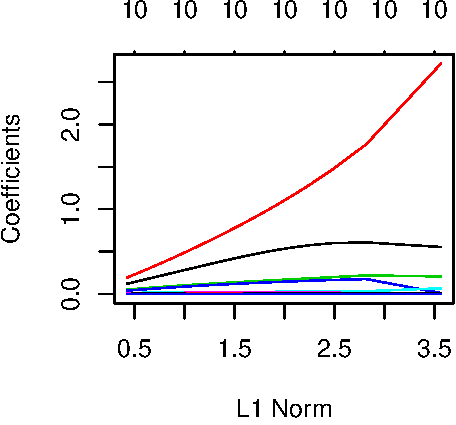
\includegraphics{sol_A4_files/figure-latex/unnamed-chunk-16-1} \end{center}

\begin{Shaded}
\begin{Highlighting}[]
\NormalTok{cv.out <-}\StringTok{ }\KeywordTok{cv.glmnet}\NormalTok{(X,y,}\DataTypeTok{alpha=}\DecValTok{0}\NormalTok{)}
\NormalTok{cv.out}\OperatorTok{$}\NormalTok{lambda.min}
\end{Highlighting}
\end{Shaded}

\begin{verbatim}
## [1] 0.4000507
\end{verbatim}

\begin{Shaded}
\begin{Highlighting}[]
\KeywordTok{plot}\NormalTok{(cv.out)}
\end{Highlighting}
\end{Shaded}

\begin{center}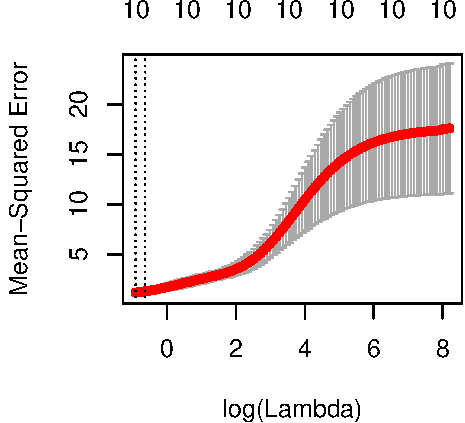
\includegraphics{sol_A4_files/figure-latex/unnamed-chunk-16-2} \end{center}

\begin{Shaded}
\begin{Highlighting}[]
\NormalTok{ridge.fit <-}\StringTok{ }\KeywordTok{glmnet}\NormalTok{(X, y, }\DataTypeTok{alpha =} \DecValTok{0}\NormalTok{, }
                    \DataTypeTok{lambda =}\NormalTok{ cv.out}\OperatorTok{$}\NormalTok{lambda.min)  }

\KeywordTok{coef}\NormalTok{(ridge.fit) }
\end{Highlighting}
\end{Shaded}

\begin{verbatim}
## 12 x 1 sparse Matrix of class "dgCMatrix"
##                                      s0
## (Intercept)                1.493577e+00
## (Intercept)                .           
## poly(x, 10, raw = TRUE)1   6.119103e-01
## poly(x, 10, raw = TRUE)2   1.859173e+00
## poly(x, 10, raw = TRUE)3   2.221955e-01
## poly(x, 10, raw = TRUE)4   1.736758e-01
## poly(x, 10, raw = TRUE)5   3.293830e-02
## poly(x, 10, raw = TRUE)6   1.120493e-02
## poly(x, 10, raw = TRUE)7   3.820191e-03
## poly(x, 10, raw = TRUE)8  -7.804433e-05
## poly(x, 10, raw = TRUE)9   2.623561e-04
## poly(x, 10, raw = TRUE)10 -2.576105e-04
\end{verbatim}

\begin{enumerate}
\def\labelenumi{(\alph{enumi})}
\setcounter{enumi}{2}
\tightlist
\item
  Repeat (b) for lasso regression instead of ridge.
\end{enumerate}

\begin{Shaded}
\begin{Highlighting}[]
\NormalTok{lasso.fit <-}\StringTok{ }\KeywordTok{glmnet}\NormalTok{(X, y, }\DataTypeTok{alpha=}\DecValTok{1}\NormalTok{, }\DataTypeTok{lambda =}\NormalTok{ grid) }
\KeywordTok{plot}\NormalTok{(lasso.fit)}
\end{Highlighting}
\end{Shaded}

\begin{center}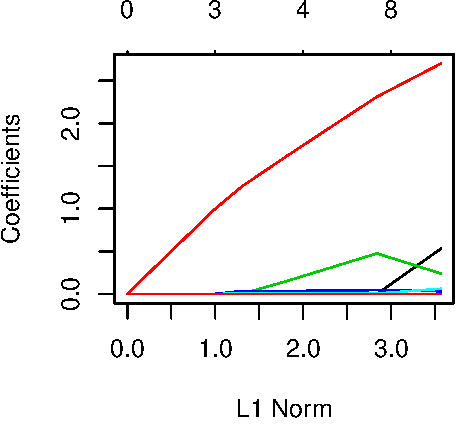
\includegraphics{sol_A4_files/figure-latex/unnamed-chunk-17-1} \end{center}

\begin{Shaded}
\begin{Highlighting}[]
\NormalTok{cv.out <-}\StringTok{ }\KeywordTok{cv.glmnet}\NormalTok{(X, y, }\DataTypeTok{alpha=}\DecValTok{1}\NormalTok{)}
\NormalTok{cv.out}\OperatorTok{$}\NormalTok{lambda.min}
\end{Highlighting}
\end{Shaded}

\begin{verbatim}
## [1] 0.0803795
\end{verbatim}

\begin{Shaded}
\begin{Highlighting}[]
\NormalTok{lasso.fit <-}\StringTok{ }\KeywordTok{glmnet}\NormalTok{(X,y,}\DataTypeTok{alpha=}\DecValTok{1}\NormalTok{, }\DataTypeTok{lambda =}\NormalTok{ cv.out}\OperatorTok{$}\NormalTok{lambda.min)  }

\KeywordTok{coef}\NormalTok{(lasso.fit) }
\end{Highlighting}
\end{Shaded}

\begin{verbatim}
## 12 x 1 sparse Matrix of class "dgCMatrix"
##                                    s0
## (Intercept)               1.180097887
## (Intercept)               .          
## poly(x, 10, raw = TRUE)1  0.380165945
## poly(x, 10, raw = TRUE)2  2.633676986
## poly(x, 10, raw = TRUE)3  0.348599739
## poly(x, 10, raw = TRUE)4  0.039359314
## poly(x, 10, raw = TRUE)5  0.032879765
## poly(x, 10, raw = TRUE)6  .          
## poly(x, 10, raw = TRUE)7  0.002025108
## poly(x, 10, raw = TRUE)8  .          
## poly(x, 10, raw = TRUE)9  .          
## poly(x, 10, raw = TRUE)10 .
\end{verbatim}

\begin{enumerate}
\def\labelenumi{(\alph{enumi})}
\setcounter{enumi}{3}
\tightlist
\item
  Plot the data y vs x and superimpose the fitted models from linear
  regression, ridge and lasso with optimal values of lambda as chosen by
  cross-validation.
\end{enumerate}

\begin{Shaded}
\begin{Highlighting}[]
\NormalTok{Xord <-}\StringTok{ }\NormalTok{X[}\KeywordTok{order}\NormalTok{(X[,}\DecValTok{2}\NormalTok{]),]}

\NormalTok{pred1 <-}\StringTok{ }\KeywordTok{predict}\NormalTok{(}\KeywordTok{lm}\NormalTok{(y}\OperatorTok{~}\KeywordTok{poly}\NormalTok{(x, }\DecValTok{10}\NormalTok{, }\DataTypeTok{raw =} \OtherTok{TRUE}\NormalTok{), }\DataTypeTok{data =}\NormalTok{ d), }
                \DataTypeTok{newdata =} \KeywordTok{data.frame}\NormalTok{(}\DataTypeTok{x =} \KeywordTok{sort}\NormalTok{(x)))}

\NormalTok{pred2 <-}\StringTok{ }\KeywordTok{predict}\NormalTok{(ridge.fit, }\DataTypeTok{newx =}\NormalTok{ Xord)}

\NormalTok{pred3 <-}\StringTok{ }\KeywordTok{predict}\NormalTok{(lasso.fit, }\DataTypeTok{newx =}\NormalTok{ Xord)}

\KeywordTok{ggplot}\NormalTok{() }\OperatorTok{+}
\StringTok{  }\KeywordTok{geom_point}\NormalTok{(}\KeywordTok{aes}\NormalTok{(x, y), }\DataTypeTok{alpha =} \FloatTok{0.8}\NormalTok{) }\OperatorTok{+}
\StringTok{  }\KeywordTok{geom_line}\NormalTok{(}\KeywordTok{aes}\NormalTok{(}\KeywordTok{sort}\NormalTok{(x), pred1), }\DataTypeTok{color =} \StringTok{"red"}\NormalTok{) }\OperatorTok{+}
\StringTok{  }\KeywordTok{geom_line}\NormalTok{(}\KeywordTok{aes}\NormalTok{(}\KeywordTok{sort}\NormalTok{(x), pred2), }\DataTypeTok{color =} \StringTok{"blue"}\NormalTok{) }\OperatorTok{+}
\StringTok{  }\KeywordTok{geom_line}\NormalTok{(}\KeywordTok{aes}\NormalTok{(}\KeywordTok{sort}\NormalTok{(x), pred3), }\DataTypeTok{color =} \StringTok{"green2"}\NormalTok{) }\OperatorTok{+}
\StringTok{  }\KeywordTok{theme_bw}\NormalTok{()}
\end{Highlighting}
\end{Shaded}

\begin{center}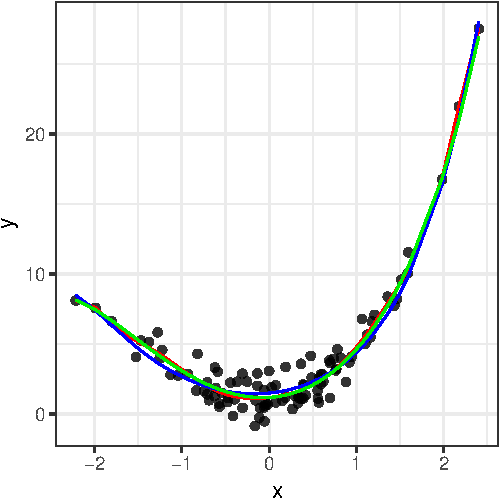
\includegraphics{sol_A4_files/figure-latex/unnamed-chunk-18-1} \end{center}

\begin{enumerate}
\def\labelenumi{\arabic{enumi}.}
\setcounter{enumi}{5}
\tightlist
\item
  Titanic data from Assignment 3:
\end{enumerate}

\begin{Shaded}
\begin{Highlighting}[]
\NormalTok{ttrain <-}\StringTok{ }\KeywordTok{read.csv}\NormalTok{(}\StringTok{"data/ttrain.csv"}\NormalTok{, }\DataTypeTok{header =} \OtherTok{TRUE}\NormalTok{, }\DataTypeTok{row.names =} \DecValTok{1}\NormalTok{)}
\NormalTok{ttest <-}\StringTok{ }\KeywordTok{read.csv}\NormalTok{(}\StringTok{"data/ttest.csv"}\NormalTok{, }\DataTypeTok{header =} \OtherTok{TRUE}\NormalTok{, }\DataTypeTok{row.names =} \DecValTok{1}\NormalTok{)}
\end{Highlighting}
\end{Shaded}

\begin{enumerate}
\def\labelenumi{(\alph{enumi})}
\tightlist
\item
  For the training data, fit a tree model using all three predictors.
  Draw the tree. Interpret the model. For the training and test data
  what proportion of survivors are missclassified? What proportion of
  those who died are missclassified? What proportion of the predicted
  survivors actually survived? What is the overall error rate for the
  training data?
\end{enumerate}

\begin{Shaded}
\begin{Highlighting}[]
\KeywordTok{library}\NormalTok{(tree)}
\NormalTok{tree <-}\StringTok{ }\KeywordTok{tree}\NormalTok{(Survived }\OperatorTok{~}\StringTok{ }\NormalTok{., }\DataTypeTok{data =}\NormalTok{ ttrain)}
\KeywordTok{summary}\NormalTok{(tree)}
\end{Highlighting}
\end{Shaded}

\begin{verbatim}
## 
## Classification tree:
## tree(formula = Survived ~ ., data = ttrain)
## Variables actually used in tree construction:
## [1] "Sex"   "Class"
## Number of terminal nodes:  3 
## Residual mean deviance:  0.9852 = 1732 / 1758 
## Misclassification error rate: 0.2107 = 371 / 1761
\end{verbatim}

\begin{Shaded}
\begin{Highlighting}[]
\KeywordTok{plot}\NormalTok{(tree)}
\KeywordTok{text}\NormalTok{(tree, }\DataTypeTok{cex =} \FloatTok{0.5}\NormalTok{, }\DataTypeTok{pretty =} \DecValTok{0}\NormalTok{)}
\end{Highlighting}
\end{Shaded}

\begin{center}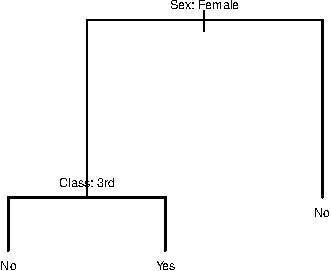
\includegraphics{sol_A4_files/figure-latex/unnamed-chunk-20-1} \end{center}

\begin{quote}
Fitted model: males have no chance of survival. For females, those in
3rd class have no chance of survival. The rest are predicted as
survived. Age is not in the model.
\end{quote}

\begin{Shaded}
\begin{Highlighting}[]
\NormalTok{prob <-}\StringTok{ }\KeywordTok{predict}\NormalTok{(tree, ttrain)[,}\DecValTok{2}\NormalTok{]}
\NormalTok{ttrain}\OperatorTok{$}\NormalTok{pred <-}\StringTok{ }\KeywordTok{factor}\NormalTok{(}\KeywordTok{ifelse}\NormalTok{(prob }\OperatorTok{<}\StringTok{ }\FloatTok{.5}\NormalTok{, }\StringTok{"No"}\NormalTok{, }\StringTok{"Yes"}\NormalTok{))}

\NormalTok{ttrain }\OperatorTok\StringTok{ }
\StringTok{  }\KeywordTok{group_by}\NormalTok{(Survived, pred) }\OperatorTok\StringTok{ }
\StringTok{  }\KeywordTok{count}\NormalTok{() }\OperatorTok\StringTok{ }
\StringTok{  }\KeywordTok{group_by}\NormalTok{(Survived) }\OperatorTok\StringTok{ }
\StringTok{  }\KeywordTok{mutate}\NormalTok{(}\DataTypeTok{perc =}\NormalTok{ scales}\OperatorTok{::}\KeywordTok{percent}\NormalTok{(n}\OperatorTok{/}\KeywordTok{sum}\NormalTok{(n)))}
\end{Highlighting}
\end{Shaded}

\begin{verbatim}
## # A tibble: 4 x 4
## # Groups:   Survived [2]
##   Survived pred      n perc 
##   <fct>    <fct> <int> <chr>
## 1 No       No     1178 98.7%
## 2 No       Yes      15 1.3% 
## 3 Yes      No      356 62.7%
## 4 Yes      Yes     212 37.3%
\end{verbatim}

\begin{Shaded}
\begin{Highlighting}[]
\NormalTok{prob <-}\StringTok{ }\KeywordTok{predict}\NormalTok{(tree, ttest)[,}\DecValTok{2}\NormalTok{]}
\NormalTok{ttest}\OperatorTok{$}\NormalTok{pred <-}\StringTok{ }\KeywordTok{factor}\NormalTok{(}\KeywordTok{ifelse}\NormalTok{(prob }\OperatorTok{<}\StringTok{ }\FloatTok{.5}\NormalTok{, }\StringTok{"No"}\NormalTok{, }\StringTok{"Yes"}\NormalTok{))}

\NormalTok{ttest }\OperatorTok\StringTok{ }
\StringTok{  }\KeywordTok{group_by}\NormalTok{(Survived, pred) }\OperatorTok\StringTok{ }
\StringTok{  }\KeywordTok{count}\NormalTok{() }\OperatorTok\StringTok{ }
\StringTok{  }\KeywordTok{group_by}\NormalTok{(Survived) }\OperatorTok\StringTok{ }
\StringTok{  }\KeywordTok{mutate}\NormalTok{(}\DataTypeTok{perc =}\NormalTok{ scales}\OperatorTok{::}\KeywordTok{percent}\NormalTok{(n}\OperatorTok{/}\KeywordTok{sum}\NormalTok{(n)))}
\end{Highlighting}
\end{Shaded}

\begin{verbatim}
## # A tibble: 4 x 4
## # Groups:   Survived [2]
##   Survived pred      n perc 
##   <fct>    <fct> <int> <chr>
## 1 No       No      292 98.3%
## 2 No       Yes       5 1.7% 
## 3 Yes      No      101 70.6%
## 4 Yes      Yes      42 29.4%
\end{verbatim}

\begin{enumerate}
\def\labelenumi{(\alph{enumi})}
\setcounter{enumi}{1}
\tightlist
\item
  Use \texttt{cv.tree} to select a pruned tree. If pruning is required,
  fit and draw the pruned tree.
\end{enumerate}

\begin{Shaded}
\begin{Highlighting}[]
\NormalTok{cvtree <-}\StringTok{ }\KeywordTok{cv.tree}\NormalTok{(tree)}

\KeywordTok{ggplot}\NormalTok{() }\OperatorTok{+}
\StringTok{  }\KeywordTok{geom_point}\NormalTok{(}\KeywordTok{aes}\NormalTok{(}\DataTypeTok{x =} \DecValTok{3}\OperatorTok{:}\DecValTok{1}\NormalTok{, }\DataTypeTok{y =} \KeywordTok{c}\NormalTok{(cvtree}\OperatorTok{$}\NormalTok{dev))) }\OperatorTok{+}
\StringTok{  }\KeywordTok{geom_line}\NormalTok{(}\KeywordTok{aes}\NormalTok{(}\DataTypeTok{x =} \DecValTok{3}\OperatorTok{:}\DecValTok{1}\NormalTok{, }\DataTypeTok{y =} \KeywordTok{c}\NormalTok{(cvtree}\OperatorTok{$}\NormalTok{dev))) }\OperatorTok{+}
\StringTok{  }\KeywordTok{theme_bw}\NormalTok{()}
\end{Highlighting}
\end{Shaded}

\begin{center}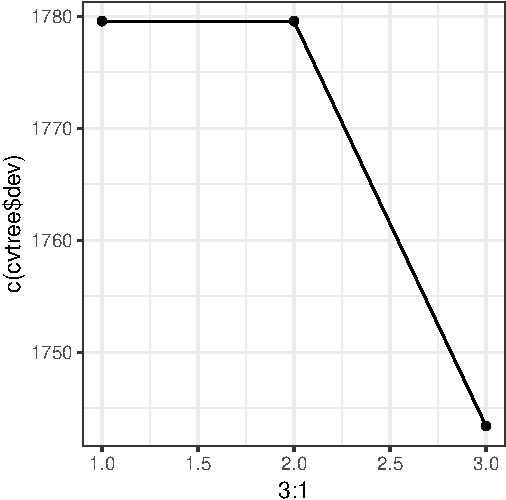
\includegraphics{sol_A4_files/figure-latex/unnamed-chunk-23-1} \end{center}

\begin{enumerate}
\def\labelenumi{(\alph{enumi})}
\setcounter{enumi}{2}
\tightlist
\item
  Fit a tree model using only Age and Class as predictors. Draw the
  tree. Interpret the model. Compare the test set results to (a).
\end{enumerate}

\begin{Shaded}
\begin{Highlighting}[]
\NormalTok{tree <-}\StringTok{ }\KeywordTok{tree}\NormalTok{(Survived }\OperatorTok{~}\StringTok{ }\NormalTok{Age }\OperatorTok{+}\StringTok{ }\NormalTok{Class, }\DataTypeTok{data =}\NormalTok{ ttrain)}
\KeywordTok{summary}\NormalTok{(tree)}
\end{Highlighting}
\end{Shaded}

\begin{verbatim}
## 
## Classification tree:
## tree(formula = Survived ~ Age + Class, data = ttrain)
## Number of terminal nodes:  4 
## Residual mean deviance:  1.148 = 2017 / 1757 
## Misclassification error rate: 0.2731 = 481 / 1761
\end{verbatim}

\begin{Shaded}
\begin{Highlighting}[]
\KeywordTok{plot}\NormalTok{(tree)}
\KeywordTok{text}\NormalTok{(tree, }\DataTypeTok{cex =} \FloatTok{0.5}\NormalTok{, }\DataTypeTok{pretty =} \DecValTok{0}\NormalTok{)}
\end{Highlighting}
\end{Shaded}

\begin{center}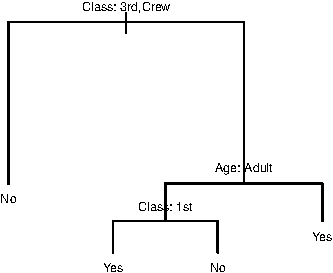
\includegraphics{sol_A4_files/figure-latex/unnamed-chunk-24-1} \end{center}

\begin{Shaded}
\begin{Highlighting}[]
\NormalTok{prob <-}\StringTok{ }\KeywordTok{predict}\NormalTok{(tree, ttrain)[,}\DecValTok{2}\NormalTok{]}
\NormalTok{ttrain}\OperatorTok{$}\NormalTok{pred <-}\StringTok{ }\KeywordTok{factor}\NormalTok{(}\KeywordTok{ifelse}\NormalTok{(prob }\OperatorTok{<}\StringTok{ }\FloatTok{.5}\NormalTok{, }\StringTok{"No"}\NormalTok{, }\StringTok{"Yes"}\NormalTok{))}

\NormalTok{ttrain }\OperatorTok\StringTok{ }
\StringTok{  }\NormalTok{dplyr}\OperatorTok{::}\KeywordTok{select}\NormalTok{(}\DecValTok{1}\OperatorTok{:}\DecValTok{3}\NormalTok{, pred) }\OperatorTok\StringTok{ }
\StringTok{  }\KeywordTok{group_by_all}\NormalTok{() }\OperatorTok\StringTok{ }
\StringTok{  }\KeywordTok{count}\NormalTok{() }\OperatorTok\StringTok{ }
\StringTok{  }\KeywordTok{arrange}\NormalTok{(pred, n)}
\end{Highlighting}
\end{Shaded}

\begin{verbatim}
## # A tibble: 14 x 5
## # Groups:   Class, Sex, Age, pred [14]
##    Class Sex    Age   pred      n
##    <fct> <fct>  <fct> <fct> <int>
##  1 Crew  Female Adult No       17
##  2 3rd   Female Child No       19
##  3 3rd   Male   Child No       37
##  4 2nd   Female Adult No       80
##  5 3rd   Female Adult No      130
##  6 2nd   Male   Adult No      132
##  7 3rd   Male   Adult No      381
##  8 Crew  Male   Adult No      686
##  9 1st   Female Child Yes       1
## 10 1st   Male   Child Yes       4
## 11 2nd   Male   Child Yes       7
## 12 2nd   Female Child Yes      13
## 13 1st   Female Adult Yes     116
## 14 1st   Male   Adult Yes     138
\end{verbatim}

\begin{quote}
Fitted model: 3rd class and crew have no chance of survival. For those
in 1st and 2nd class children are predicted to have survived. Adults in
1st class are predicted to have survived, but those in the 2nd did not.
\end{quote}

\begin{Shaded}
\begin{Highlighting}[]
\NormalTok{prob <-}\StringTok{ }\KeywordTok{predict}\NormalTok{(tree, ttest)[,}\DecValTok{2}\NormalTok{]}
\NormalTok{ttest}\OperatorTok{$}\NormalTok{pred <-}\StringTok{ }\KeywordTok{factor}\NormalTok{(}\KeywordTok{ifelse}\NormalTok{(prob }\OperatorTok{<}\StringTok{ }\FloatTok{.5}\NormalTok{, }\StringTok{"No"}\NormalTok{, }\StringTok{"Yes"}\NormalTok{))}

\NormalTok{ttest }\OperatorTok\StringTok{ }
\StringTok{  }\KeywordTok{group_by}\NormalTok{(Survived, pred) }\OperatorTok\StringTok{ }
\StringTok{  }\KeywordTok{count}\NormalTok{() }\OperatorTok\StringTok{ }
\StringTok{  }\KeywordTok{group_by}\NormalTok{(Survived) }\OperatorTok\StringTok{ }
\StringTok{  }\KeywordTok{mutate}\NormalTok{(}\DataTypeTok{perc =}\NormalTok{ scales}\OperatorTok{::}\KeywordTok{percent}\NormalTok{(n}\OperatorTok{/}\KeywordTok{sum}\NormalTok{(n)))}
\end{Highlighting}
\end{Shaded}

\begin{verbatim}
## # A tibble: 4 x 4
## # Groups:   Survived [2]
##   Survived pred      n perc 
##   <fct>    <fct> <int> <chr>
## 1 No       No      271 91.2%
## 2 No       Yes      26 8.8% 
## 3 Yes      No       99 69.2%
## 4 Yes      Yes      44 30.8%
\end{verbatim}

\begin{enumerate}
\def\labelenumi{(\alph{enumi})}
\setcounter{enumi}{3}
\tightlist
\item
  Fit a random forest model (using \texttt{randomForest}) using all
  three predictors and compare the test set results to (a) and (c).
  Which variables are important?
\end{enumerate}

\begin{Shaded}
\begin{Highlighting}[]
\KeywordTok{library}\NormalTok{(randomForest)}
\NormalTok{bag <-}\StringTok{ }\KeywordTok{randomForest}\NormalTok{(Survived }\OperatorTok{~}\StringTok{ }\NormalTok{., }\DataTypeTok{data =}\NormalTok{ ttrain)}
\KeywordTok{varImpPlot}\NormalTok{(bag)}
\end{Highlighting}
\end{Shaded}

\begin{center}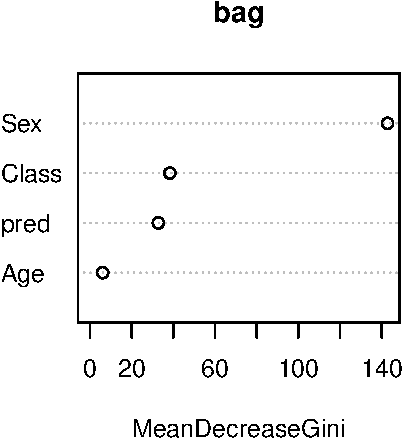
\includegraphics{sol_A4_files/figure-latex/unnamed-chunk-26-1} \end{center}

\begin{Shaded}
\begin{Highlighting}[]
\NormalTok{ttest}\OperatorTok{$}\NormalTok{pred <-}\StringTok{ }\KeywordTok{predict}\NormalTok{(bag, }\DataTypeTok{newdata =}\NormalTok{ ttest)}

\NormalTok{ttest }\OperatorTok\StringTok{ }
\StringTok{  }\KeywordTok{group_by}\NormalTok{(Survived, pred) }\OperatorTok\StringTok{ }
\StringTok{  }\KeywordTok{count}\NormalTok{() }\OperatorTok\StringTok{ }
\StringTok{  }\KeywordTok{group_by}\NormalTok{(Survived) }\OperatorTok\StringTok{ }
\StringTok{  }\KeywordTok{mutate}\NormalTok{(}\DataTypeTok{perc =}\NormalTok{ scales}\OperatorTok{::}\KeywordTok{percent}\NormalTok{(n}\OperatorTok{/}\KeywordTok{sum}\NormalTok{(n)))}
\end{Highlighting}
\end{Shaded}

\begin{verbatim}
## # A tibble: 4 x 4
## # Groups:   Survived [2]
##   Survived pred      n perc 
##   <fct>    <fct> <int> <chr>
## 1 No       No      292 98.3%
## 2 No       Yes       5 1.7% 
## 3 Yes      No       96 67.1%
## 4 Yes      Yes      47 32.9%
\end{verbatim}

\begin{enumerate}
\def\labelenumi{\arabic{enumi}.}
\setcounter{enumi}{6}
\tightlist
\item
  Heart data: binary outcome AHD for 303 patients who presented with
  chest pain. An outcome value of Yes indicates the presence of heart
  disease, while No means no heart disease.
\end{enumerate}

There are 13 predictors including Age, Sex, Chol (a cholesterol
measurement), and other heart and lung function measurements.

Fit a support vector machine with a radial kernel to this data. Use
cross validation to tune the \(\lambda\) and cost parameters (see
function \texttt{tune()} in e1071 library). How does your result (test
error) compare to the test error in the notes (obtained using trees and
random forrests)?

\begin{Shaded}
\begin{Highlighting}[]
\KeywordTok{set.seed}\NormalTok{(}\DecValTok{2019}\NormalTok{)}
\NormalTok{heart <-}\StringTok{ }\KeywordTok{read.csv}\NormalTok{(}\StringTok{"data/heart.csv"}\NormalTok{, }\DataTypeTok{row.names=}\DecValTok{1}\NormalTok{) }\OperatorTok\StringTok{ }\KeywordTok{na.omit}\NormalTok{()}

\NormalTok{heart <-}\StringTok{  }\NormalTok{heart }\OperatorTok\StringTok{ }
\StringTok{  }\KeywordTok{mutate}\NormalTok{(}\DataTypeTok{part =} \KeywordTok{ifelse}\NormalTok{(}\KeywordTok{runif}\NormalTok{(}\KeywordTok{nrow}\NormalTok{(.)) }\OperatorTok{>}\StringTok{ }\FloatTok{0.66}\NormalTok{, }\StringTok{"test"}\NormalTok{, }\StringTok{"train"}\NormalTok{))}

\NormalTok{heart }\OperatorTok\StringTok{ }
\StringTok{  }\NormalTok{janitor}\OperatorTok{::}\KeywordTok{tabyl}\NormalTok{(part)}
\end{Highlighting}
\end{Shaded}

\begin{verbatim}
##   part   n   percent
##   test  92 0.3097643
##  train 205 0.6902357
\end{verbatim}

\begin{Shaded}
\begin{Highlighting}[]
\NormalTok{train <-}\StringTok{ }\NormalTok{heart }\OperatorTok\StringTok{ }\KeywordTok{filter}\NormalTok{(part }\OperatorTok{==}\StringTok{ "train"}\NormalTok{) }\OperatorTok\StringTok{ }\NormalTok{dplyr}\OperatorTok{::}\KeywordTok{select}\NormalTok{(}\OperatorTok{-}\NormalTok{part)}
\NormalTok{test <-}\StringTok{ }\NormalTok{heart }\OperatorTok\StringTok{ }\KeywordTok{filter}\NormalTok{(part }\OperatorTok{==}\StringTok{ "test"}\NormalTok{) }\OperatorTok\StringTok{ }\NormalTok{dplyr}\OperatorTok{::}\KeywordTok{select}\NormalTok{(}\OperatorTok{-}\NormalTok{part)}


\KeywordTok{library}\NormalTok{(e1071)}

\NormalTok{fit.svm <-}\StringTok{ }\KeywordTok{svm}\NormalTok{(AHD }\OperatorTok{~}\StringTok{ }\NormalTok{., }\DataTypeTok{data =}\NormalTok{ train, }\DataTypeTok{kernel =} \StringTok{"radial"}\NormalTok{)}
\KeywordTok{summary}\NormalTok{(fit.svm)}
\end{Highlighting}
\end{Shaded}

\begin{verbatim}
## 
## Call:
## svm(formula = AHD ~ ., data = train, kernel = "radial")
## 
## 
## Parameters:
##    SVM-Type:  C-classification 
##  SVM-Kernel:  radial 
##        cost:  1 
##       gamma:  0.05882353 
## 
## Number of Support Vectors:  117
## 
##  ( 57 60 )
## 
## 
## Number of Classes:  2 
## 
## Levels: 
##  No Yes
\end{verbatim}

\begin{Shaded}
\begin{Highlighting}[]
\NormalTok{test}\OperatorTok{$}\NormalTok{pred <-}\StringTok{ }\KeywordTok{predict}\NormalTok{(fit.svm, }\DataTypeTok{newdata =}\NormalTok{ test)}

\NormalTok{test }\OperatorTok\StringTok{ }
\StringTok{  }\KeywordTok{group_by}\NormalTok{(AHD, pred) }\OperatorTok\StringTok{ }
\StringTok{  }\KeywordTok{count}\NormalTok{()}
\end{Highlighting}
\end{Shaded}

\begin{verbatim}
## # A tibble: 4 x 3
## # Groups:   AHD, pred [4]
##   AHD   pred      n
##   <fct> <fct> <int>
## 1 No    No       42
## 2 No    Yes       3
## 3 Yes   No       12
## 4 Yes   Yes      35
\end{verbatim}

\begin{Shaded}
\begin{Highlighting}[]
\NormalTok{tune.out <-}\StringTok{ }\KeywordTok{tune}\NormalTok{(svm,AHD}\OperatorTok{~}\NormalTok{., }\DataTypeTok{data =}\NormalTok{ train, }\DataTypeTok{kernel =} \StringTok{"radial"}\NormalTok{, }
                 \DataTypeTok{ranges =} \KeywordTok{list}\NormalTok{(}\DataTypeTok{cost =} \DecValTok{10}\OperatorTok{^}\KeywordTok{seq}\NormalTok{(}\OperatorTok{-}\DecValTok{1}\NormalTok{, }\DecValTok{6}\NormalTok{, }\DataTypeTok{by =} \DecValTok{1}\NormalTok{), }
                               \DataTypeTok{gamma =} \DecValTok{10}\OperatorTok{^}\KeywordTok{seq}\NormalTok{(}\OperatorTok{-}\DecValTok{6}\NormalTok{, }\DecValTok{1}\NormalTok{, }\DataTypeTok{by =} \DecValTok{1}\NormalTok{)))}
\NormalTok{tune.out}
\end{Highlighting}
\end{Shaded}

\begin{verbatim}
## 
## Parameter tuning of 'svm':
## 
## - sampling method: 10-fold cross validation 
## 
## - best parameters:
##   cost gamma
##  1e+05 1e-04
## 
## - best performance: 0.1554762
\end{verbatim}

\begin{Shaded}
\begin{Highlighting}[]
\NormalTok{fit.svm <-}\StringTok{ }\KeywordTok{svm}\NormalTok{(AHD}\OperatorTok{~}\NormalTok{., }\DataTypeTok{data =}\NormalTok{ train, }\DataTypeTok{kernel =} \StringTok{"radial"}\NormalTok{, }
               \DataTypeTok{cost =} \DecValTok{10000}\NormalTok{, }\DataTypeTok{gamma =} \FloatTok{0.00001}\NormalTok{)}
\KeywordTok{summary}\NormalTok{(fit.svm)}
\end{Highlighting}
\end{Shaded}

\begin{verbatim}
## 
## Call:
## svm(formula = AHD ~ ., data = train, kernel = "radial", cost = 10000, 
##     gamma = 1e-05)
## 
## 
## Parameters:
##    SVM-Type:  C-classification 
##  SVM-Kernel:  radial 
##        cost:  10000 
##       gamma:  1e-05 
## 
## Number of Support Vectors:  82
## 
##  ( 40 42 )
## 
## 
## Number of Classes:  2 
## 
## Levels: 
##  No Yes
\end{verbatim}

\begin{Shaded}
\begin{Highlighting}[]
\NormalTok{test}\OperatorTok{$}\NormalTok{pred <-}\StringTok{ }\KeywordTok{predict}\NormalTok{(fit.svm, }\DataTypeTok{newdata =}\NormalTok{ test)}


\NormalTok{test }\OperatorTok\StringTok{ }
\StringTok{  }\KeywordTok{group_by}\NormalTok{(AHD, pred) }\OperatorTok\StringTok{ }
\StringTok{  }\KeywordTok{count}\NormalTok{()}
\end{Highlighting}
\end{Shaded}

\begin{verbatim}
## # A tibble: 4 x 3
## # Groups:   AHD, pred [4]
##   AHD   pred      n
##   <fct> <fct> <int>
## 1 No    No       42
## 2 No    Yes       3
## 3 Yes   No       11
## 4 Yes   Yes      36
\end{verbatim}

\begin{Shaded}
\begin{Highlighting}[]
\NormalTok{bag <-}\StringTok{ }\KeywordTok{randomForest}\NormalTok{(AHD }\OperatorTok{~}\StringTok{ }\NormalTok{., }\DataTypeTok{data =}\NormalTok{ train)}
\NormalTok{test}\OperatorTok{$}\NormalTok{pred <-}\StringTok{ }\KeywordTok{predict}\NormalTok{(bag, test)}

\NormalTok{test }\OperatorTok\StringTok{ }
\StringTok{  }\KeywordTok{group_by}\NormalTok{(AHD, pred) }\OperatorTok\StringTok{ }
\StringTok{  }\KeywordTok{count}\NormalTok{()}
\end{Highlighting}
\end{Shaded}

\begin{verbatim}
## # A tibble: 4 x 3
## # Groups:   AHD, pred [4]
##   AHD   pred      n
##   <fct> <fct> <int>
## 1 No    No       40
## 2 No    Yes       5
## 3 Yes   No       11
## 4 Yes   Yes      36
\end{verbatim}


\end{document}
